\documentclass[]{article}
\usepackage{ctex,hyperref}% 输出汉字
\usepackage{amsmath,amssymb,amsfonts}
\usepackage{amsthm,amsmath,amssymb}
\usepackage{mathrsfs}
%opening
\usepackage{setspace}
\usepackage{lipsum}
\usepackage{graphicx}% 图片插入宏包
\usepackage{subfigure}% 并排子图
\usepackage{float}% 浮动环境,用于调整图片位置
\usepackage[export]{adjustbox}% 防止过宽的图片
\usepackage{amsmath}
\usepackage{extarrows}
\graphicspath{{Figures/}}%文章所用图片在当前目录下的 Figures目录
\title{Hartree-Fock方法}
\author{步允霆}

\begin{document}
	
	\maketitle
	
\section{自旋轨道的积分表示}
分子轨道使用自旋轨道(spin orbital)表示,其中包含空间函数(spatial function)与自旋函数(spin function),以$\alpha$自旋为例:
\begin{equation}
	\chi_i(\mathbf{x})=\psi_j(\mathbf{r})\alpha(\omega)
\end{equation}

我们约定以下符号来表示电子积分,之后我们将反复用到。

对于自旋轨道:
\begin{align}
	&[i|h|j] = \left\langle i|h|j\right\rangle  = \int \mathrm{d}\mathbf{x_1}\chi_i^*(\mathbf{x_1}) h(\mathbf{r_1})\chi_j(\mathbf{x_1})\\
	&\left\langle ij|kl\right\rangle = \int \mathrm{d}\mathbf{x_1}\mathrm{d}\mathbf{x_2}\chi_i^*(\mathbf{x_1})\chi_j^*(\mathbf{x_2})r_{12}^{-1}\chi_k(\mathbf{x_1})\chi_l(\mathbf{x_2}) \\
	&[ij|kl]= \int \mathrm{d}\mathbf{x_1}\mathrm{d}\mathbf{x_2}\chi_i^*(\mathbf{x_1})\chi_j(\mathbf{x_1})r_{12}^{-1}\chi_k^*(\mathbf{x_2})\chi_l(\mathbf{x_2})\\
	&\left\langle ij||kl \right\rangle = \left\langle ij|kl\right\rangle -\left\langle ij|lk \right\rangle
\end{align}

对于空间轨道:
\begin{align}
	&(i|h|j)=h_{ij}=\int \mathrm{d}\mathbf{r_1}\psi_i^*(\mathbf{r_1}) h(\mathbf{r_1})\psi_j(\mathbf{r_1})\\
	&(ij|kl)=(\psi_i\psi_j|\psi_k\psi_l)=\int \mathrm{d}\mathbf{r_1}\mathrm{d}\mathbf{r_2}\psi_i^*(\mathbf{r_1})\psi_j(\mathbf{r_1})r_{12}^{-1}\psi_k^*(\mathbf{r_2})\psi_l(\mathbf{r_2})\\
	&J_{ij}=(ii|jj)\quad Coulomb\ integrals\\
	&K_{ij}=(ij|ji)\quad Exchange\ integrals
\end{align}

\section{Slater-Condon规则}

上面的积分表示中,出现了$h(\mathbf{r_1})$与$r_{12}^{-1}$两种算符,分别为单电子算符与双电子算符。对于含有N个电子的体系,用Slater行列式表示分子波函数,可以写为$|K\rangle = |\cdots \chi_m \chi_n \cdots \rangle $或$|K\rangle = |\cdots mn \cdots \rangle $。如果用$\mathscr{H}$哈密顿算符,则基态能量的期望值为$E_0=\left\langle K|\mathscr{H}|K \right\rangle $,Slater-Condon规则利用行列式展开,将矩阵元进行了简化,规则如下(该规则还有很多种其他情况,我们这里不考虑):
\begin{align}
	&\left\langle K|h|K \right\rangle =\sum\limits_m^N [m|h|m]=\sum\limits_m^N\left\langle m|h|m \right\rangle \\
	&\left\langle K|r_{12}^{-1}|K \right\rangle = \frac{1}{2}\sum\limits_m^N \sum\limits_n^N [mm|nn]-[mn|nm]=\frac{1}{2}\sum\limits_m^N \sum\limits_n^N \left\langle mn||mn \right\rangle 
\end{align}

因此,基态能量可以写为:
\begin{equation}
	E_0 = \sum\limits_m^N [m|h|m]+\frac{1}{2}\sum\limits_m^N \sum\limits_n^N [mm|nn]-[mn|nm]
\end{equation}
\section{Hartree-Fock方程的推导}
\subsection{单行列式的能量最小化}
给定一个单行列式$|\Psi_0\rangle=|\chi_1\chi_2\cdots\chi_a\chi_b\cdots\chi_N\rangle$,能量为$E_0=\left\langle \Psi_0|\mathscr{H}|\Psi_0\right\rangle $,为推导Hartree-Fock方程,我们需要最小化$E_0\left[ \left\lbrace \chi_a\right\rbrace\right] $(这是一种泛函的表示)。自旋轨道的约束条件是要符合正交归一化:
\begin{equation}
	\int \mathrm{d}\mathbf{x_1}\chi_a^*(1)\chi_b(1)=[a|b]=\delta_{ab}
\end{equation}
可以改写为:
\begin{equation}
	[a|b]-\delta_{ab}=0
\end{equation}

我们用Lagrange乘数法,构造泛函:
\begin{equation}
	\mathscr{L}\left[ \left\lbrace \chi_a\right\rbrace \right]=E_0\left[ \left\lbrace \chi_a\right\rbrace\right]-\sum\limits_a^N\sum\limits_b^N\varepsilon_{ba}([a|b]-\delta_{ab})
\end{equation}
其中,如上节所述,$E_0$的表达式为:
\begin{equation}
	E_0\left[ \left\lbrace \chi_a\right\rbrace\right] = \sum\limits_a^N [a|h|a]+\frac{1}{2}\sum\limits_a^N \sum\limits_b^N [aa|bb]-[ab|ba]
\end{equation}
$\varepsilon_{ba}$是Lagrange乘子。因为$\mathscr{L}$是实的而且$[a|b]=[b|a]^*$,因此Lagrange乘子一定是Hermitian矩阵的元素,即$\varepsilon_{ba}=\varepsilon_{ab}^*$,证明如下:
\begin{equation}
	\mathscr{L}\left[ \left\lbrace \chi_a\right\rbrace \right]=E_0\left[ \left\lbrace \chi_a\right\rbrace\right]-\sum\limits_a^N\sum\limits_b^N\varepsilon_{ba}([a|b]-\delta_{ab})
\end{equation}
取共轭,我们有
\begin{equation}
	\mathscr{L}\left[ \left\lbrace \chi_a\right\rbrace \right]^*=E_0\left[ \left\lbrace \chi_a\right\rbrace\right]^*-\sum\limits_a^N\sum\limits_b^N\varepsilon_{ba}^*([a|b]^*-\delta_{ab}^*)
\end{equation}
化简
\begin{equation}
	\mathscr{L}\left[ \left\lbrace \chi_a\right\rbrace \right]=E_0\left[ \left\lbrace \chi_a\right\rbrace\right]-\sum\limits_a^N\sum\limits_b^N\varepsilon_{ba}^*([b|a]-\delta_{ab})
\end{equation}
因此
\begin{equation}
	\sum\limits_a^N\sum\limits_b^N\varepsilon_{ba}([a|b]-\delta_{ab})=\sum\limits_a^N\sum\limits_b^N\varepsilon_{ba}^*([b|a]-\delta_{ab})=\sum\limits_b^N\sum\limits_a^N\varepsilon_{ab}^*([a|b]-\delta_{ab})
\end{equation}
故得
\begin{equation}
	\varepsilon_{ba}=\varepsilon_{ab}^*
\end{equation}

对$\mathscr{L}$进行变分并等于0,则:
\begin{equation}
	\delta\mathscr{L}=\delta E_0-\sum\limits_a^N\sum\limits_b^N\varepsilon_{ba}\delta[a|b]
\end{equation}
因为
\begin{equation}
	\delta[a|b]=[\delta\chi_a|\chi_b]+[\chi_a|\delta\chi_b]
\end{equation}
展开$\delta E_0$得
\begin{align}
	\delta E_0=&\sum\limits_a^N[\delta \chi_a|h|\chi_a]+[\chi_a|h|\delta\chi_a]\nonumber\\
	&+\frac{1}{2}\sum\limits_a^N\sum\limits_b^N[\delta\chi_a\chi_a|\chi_b\chi_b]+[\chi_a\delta\chi_a|\chi_b\chi_b]+[\chi_a\chi_a|\delta\chi_b\chi_b]+[\chi_a\chi_a|\chi_b\delta\chi_b]\nonumber\\
	&-\frac{1}{2}\sum\limits_a^N\sum\limits_b^N[\delta\chi_a\chi_b|\chi_b\chi_a]+[\chi_a\delta\chi_b|\chi_b\chi_a]+[\chi_a\chi_b|\delta\chi_b\chi_a]+[\chi_a\chi_b|\chi_b\delta\chi_a]
\end{align}
简化
\begin{equation}
	\delta E_0=\sum\limits_a^N[\delta \chi_a|h|\chi_a]+\sum\limits_a^N\sum\limits_b^N[\delta\chi_a\chi_a|\chi_b\chi_b]-[\delta\chi_a\chi_b|\chi_b\chi_a]+\mathrm{complex\ conjugate}
\end{equation}
证明思路如下
\begin{align}
	[\chi_a\delta\chi_a|\chi_b\chi_b]
	&=\int\mathrm{d}\mathbf{x_1}\mathrm{d}\mathbf{x_2}\chi_a^*(1)\delta\chi_a(1)r^{-1}_{12}\chi_b^*(2)\chi_b(2)\nonumber\\
	&=[\int\mathrm{d}\mathbf{x_1}\mathrm{d}\mathbf{x_2}\delta\chi_a^*(1)\chi_a(1)r^{-1}_{12}\chi_b^*(2)\chi_b(2)]^*\nonumber\\
	&=[\delta\chi_a\chi_a|\chi_b\chi_b]
\end{align}
同样的
\begin{align}
	\sum\limits_{ab}\varepsilon_{ba}([\delta\chi_a|\chi_b]+[\chi_a|\delta\chi_b])
	&=\sum\limits_{ab}\varepsilon_{ba}[\delta\chi_a|\chi_b]+\sum\limits_{ab}\varepsilon_{ab}[\chi_b|\delta\chi_a]\nonumber\\
	&=\sum\limits_{ab}\varepsilon_{ba}[\delta\chi_a|\chi_b]+\sum\limits_{ab}\varepsilon_{ba}^*[\chi_a|\delta\chi_b]^*\nonumber\\
	&=\sum\limits_{ab}\varepsilon_{ba}[\delta\chi_a|\chi_b]+\mathrm{complex\ conjugate}
\end{align}
因此,式(18)表示为
\begin{align}
	\delta\mathscr{L}=
	&\sum\limits_a^N[\delta \chi_a|h|\chi_a]+\sum\limits_a^N\sum\limits_b^N[\delta\chi_a\chi_a|\chi_b\chi_b]-[\delta\chi_a\chi_b|\chi_b\chi_a]\nonumber\\
	&-\sum\limits_a^N\sum\limits_b^N\varepsilon_{ba}[\delta\chi_a|\chi_b]+\mathrm{complex\ conjugate}=0
\end{align}

再接下来的简化之前,我们先介绍两种算符——Coulomb算符与交换算符。

定义Coulomb算符:
\begin{equation}
	\mathscr{J}_b(1)=\int\mathrm{d}\mathbf{x_2}\chi_b^*(2)r^{-1}_{12}\chi_b(2)
\end{equation}

定义交换算符:
\begin{equation}
	\mathscr{K}_b(1)\chi_a(1)=\left[\int\mathrm{d}\mathbf{x_2}\chi_b^*(2)r^{-1}_{12}\chi_a(2) \right] \chi_b(1)
\end{equation}
与Coulomb算符比较:
\begin{equation}
	\mathscr{J}_b(1)\chi_a(1)=\left[ \int\mathrm{d}\mathbf{x_2}\chi_b^*(2)r^{-1}_{12}\chi_b(2)\right] \chi_a(1)
\end{equation}

可以看出来,$\mathscr{K}_b(1)$作用在$\chi_a(1)$时会涉及到坐标交换:与式(27)相比,式(26)中$r^{-1}_{12}$右边的电
子 1 和 2 的坐标交换了顺序.

对于$\chi_a$的Coulomb势与交换势的期望值,就是所谓的Coulomb积分与交换积分:
\begin{equation}
	\left\langle\chi_a(1)|\mathscr{J}_b(1)|\chi_a(1) \right\rangle =\int\mathrm{d}\mathbf{x_1}\mathrm{d}\mathbf{x_2}\chi_a^*(1)\chi_a(1)r^{-1}_{12}\chi_b^*(1)\chi_b(1)=[aa|bb]
\end{equation}
\begin{equation}
	\left\langle\chi_a(1)|\mathscr{K}_b(1)|\chi_a(1) \right\rangle =\int\mathrm{d}\mathbf{x_1}\mathrm{d}\mathbf{x_2}\chi_a^*(1)\chi_b(1)r^{-1}_{12}\chi_b^*(1)\chi_a(1)=[ab|ba]
\end{equation}

我们继续回到HF的推导中。将式(24)中的$\delta\chi_a^*(1)$提出,并用Coulomb算符与交换算符改写,得
\begin{align}
	\delta\mathscr{L}=
	&\sum\limits_a^N\int\mathrm{d}\mathbf{x_1}\delta\chi_a^*(1)\left[ h(1)\chi_a(1)+\sum\limits_b^N\left( \mathscr{J}_b(1)-\mathscr{K}_b(1)\right) \chi_a(1)-\sum\limits_b^N\varepsilon_{ba}\chi_b(1)\right] \nonumber\\
	&+\mathrm{complex\ conjugate}=0
\end{align}
因为$\delta\chi_a^*(1)$是任意的, 那么上面方括号中的量对所有指标 a 都为零。也就是
\begin{equation}
	\left[ h(1)+\sum\limits_b^N\mathscr{J}_b(1)-\mathscr{K}_b(1)\right]\chi_a(1)=\sum\limits_b^N\varepsilon_{ba}\chi_b(1)
\end{equation}
定义Fock算符:
\begin{equation}
	f(1)=h(1)+\sum\limits_b^N\mathscr{J}_b(1)-\mathscr{K}_b(1)
\end{equation}
因此式(31)可写为:
\begin{equation}
	f|\chi_a\rangle=\sum\limits_b^N\varepsilon_{ba}|\chi_b\rangle
\end{equation}

这个结果第一眼看来可能有些奇怪, 因为它不是标准的本征值形式。 原
因就是任意一个由自旋轨道$\left\lbrace \chi_a\right\rbrace $ 构成的单行列式波函数$|\Psi_0\rangle$在自旋轨道本身上仍然
留有一定的任意性:可以混合这些自旋轨道而不改变期望值$E_0=\left\langle K|\mathscr{H}|K \right\rangle $。在导出
Hartree-Fock方程的正则形式前, 我们需要考虑自旋轨道之间的的酉变换。
\subsection{正则Hartree-Fock方程}
上节所述,我们推导的HF方程并非标准的本征方程,这节的目的就是为了解决这个问题。

现在考虑一组新的自旋轨道$\left\lbrace \chi_a'\right\rbrace $,它是通过如下的酉变换从旧的自旋轨道$\left\lbrace \chi_a\right\rbrace $所得:
\begin{equation}
	\chi_a'=\sum\limits_b^N\chi_bU_{ba}
\end{equation}
所谓酉变换(unitary transformation), 就是满足如下关系的变换:
\begin{equation}
	\mathbf{U^{\dagger}}=\mathbf{U^{-1}}
\end{equation}
它能保持被变换基的正交归一性。也就是说,若从一组正交归一的自旋轨道 $\left\lbrace \chi_a\right\rbrace $出发, 经该变换得到一组新的自旋轨道$\left\lbrace \chi_a'\right\rbrace $, 则后者也是正交归一的. 下面定义一个方阵$\mathbf{A}$:
\begin{equation}
	\mathbf{A}=\begin{pmatrix}
		\chi_1(1)&\chi_2(1)&\cdots&\chi_a(1)&\cdots&\chi_N(1)\\
		\chi_1(2)&\chi_2(2)&\cdots&\chi_a(2)&\cdots&\chi_N(2)\\
		\vdots	 &\vdots   &	  &\vdots   &      &\vdots\\
		\chi_1(N)&\chi_2(N)&\cdots&\chi_a(N)&\cdots&\chi_N(N)\\
	\end{pmatrix}
\end{equation}
以使波函数$|\Psi_0\rangle$就是该矩阵的归一化行列式:
\begin{equation}
	|\Psi_0\rangle=(N!)^{-1/2}\mathrm{det}(\mathbf{A})
\end{equation}
由$\mathbf{A}$经变换所得的包含变换后的自旋轨道的$\mathbf{A'}$如下
\begin{align}
	\mathbf{A'}=\mathbf{AU}
	&=
	\begin{pmatrix}
		\chi_1(1)&\chi_2(1)&\cdots&\chi_a(1)&\cdots&\chi_N(1)\\
		\chi_1(2)&\chi_2(2)&\cdots&\chi_a(2)&\cdots&\chi_N(2)\\
		\vdots	 &\vdots   &	  &\vdots   &      &\vdots\\
		\chi_1(N)&\chi_2(N)&\cdots&\chi_a(N)&\cdots&\chi_N(N)\\
	\end{pmatrix}
	\begin{pmatrix}
		U_{11}&U_{12}&\cdots&U_{1N}\\
		U_{21}&U_{22}&\cdots&U_{2N}\\
		\vdots&\vdots&	    &\vdots\\
		U_{N1}&U_{N2}&\cdots&U_{NN}\\
	\end{pmatrix}\nonumber\\
	&=
	\begin{pmatrix}
		\chi_1'(1)&\chi_2'(1)&\cdots&\chi_a'(1)&\cdots&\chi_N'(1)\\
		\chi_1'(2)&\chi_2'(2)&\cdots&\chi_a'(2)&\cdots&\chi_N'(2)\\
		\vdots	 &\vdots   &	  &\vdots   &      &\vdots\\
		\chi_1'(N)&\chi_2'(N)&\cdots&\chi_a'(N)&\cdots&\chi_N'(N)\\
	\end{pmatrix}
\end{align}
因为
\begin{equation}
	\mathrm{det}(\mathbf{AB})=\mathrm{det}(\mathbf{A})\mathrm{det}(\mathbf{B})
\end{equation}
变换后的自旋轨道构成的行列式与旧轨道的行列式有如下关系:
\begin{equation}
	\mathrm{det}(\mathbf{A'})=\mathrm{det}(\mathbf{U})\mathrm{det}(\mathbf{A})
\end{equation}
或者等价于
\begin{equation}
	|\Psi_0'\rangle=\mathrm{det}(\mathbf{U})|\Psi_0\rangle
\end{equation}
又因为
\begin{equation}
	\mathrm{det}(\mathbf{U^{\dagger}U})=1
\end{equation}
我们有
\begin{equation}
	\mathrm{det}(\mathbf{U^{\dagger}U})=\mathrm{det}(\mathbf{U^{\dagger}})\mathrm{det}(\mathbf{U})=(\mathrm{det}(\mathbf{U}))^*\mathrm{det}(\mathbf{U})=|\mathrm{det}(\mathbf{U})|^2=\mathrm{det}(\mathbf{1})=1
\end{equation}
因此
\begin{equation}
	\mathrm{det}(\mathbf{U})=e^{\mathrm{i}\phi}
\end{equation}

所以变换后的行列式$|\Psi_0'\rangle$与原来的行列式只差一个相因子. 若 $\mathrm{U}$是实矩阵, 则这个相因子的值只能取±1. 由于所有的可观测性质仅依赖于$|\Psi|^2$, 所以在任何地方, 由$\left\lbrace \chi_a\right\rbrace $组成的原式波函数和由$\left\lbrace \chi_a'\right\rbrace $组成的变换后的波函数都是等同的. 在单行列式波函数下, 所有期望值在自旋轨道的任意酉变换下都不变.

我们利用单行列式在自旋轨道酉变换下不变的性质, 可以简化式(33), 将其改写为关于一组特定轨道的本征值方程。但首先需确定以上酉变换对Fock算符和Lagrange乘子的作用效果。Fock算符中依赖于自旋轨道的部分是Coulomb和交换算符。经过变换后的库伦算符之和为:
\begin{align}
	\sum\limits_a\mathscr{J}'_a(1)
	&=\sum\limits_a\int\mathrm{d}\mathbf{x_2}\chi_a'^*(2)r^{-1}_{12}\chi_a'(2)\nonumber\\
	&=\sum\limits_{bc}\left[ \sum\limits_aU^*_{ba}U_{ca}\right] \sum\limits_b\int\mathrm{d}\mathbf{x_2}\chi_b^*(2)r^{-1}_{12}\chi_c(2)
\end{align}
但是
\begin{equation}
	\sum\limits_aU^*_{ba}U_{ca}=(\mathbf{U^{\dagger}U})_{cb}=\delta_{cb}
\end{equation}
所以
\begin{equation}
	\sum\limits_a\mathscr{J}'_a(1)=\sum\limits_b\int\mathrm{d}\mathbf{x_2}\chi_b^*(2)r^{-1}_{12}\chi_b(2)=\sum\limits_b\mathscr{J}'_b(1)
\end{equation}
因此库伦算符在自旋轨道的酉变换下不变。

以相同的方式易证交换算符之和在自旋轨道的任意酉变换下不变, 因而 Fock 算符也不变:
\begin{equation}
	f'(1)=f(1)
\end{equation}

现在来确定酉变换对Lagrange乘子的作用。将 (31) 左乘$\langle\chi_c|$ 就可证明 Lagrange乘子是Fock算符的矩阵元:
\begin{equation}
	\left\langle \chi_c|f|\chi_a\right\rangle =\sum\limits^N_b\varepsilon_{ba}\left\langle \chi_c|\chi_a\right\rangle=\varepsilon_{ca}
\end{equation}
因此
\begin{align}
	\varepsilon'_{ab}
	&=\int\mathrm{d}\mathbf{x_1}\chi'^*_a(1)f(1)\chi'_b(1)\nonumber\\
	&=\sum\limits_{cd}U^*_{ca}U_{db}\int\mathrm{d}\mathbf{x_1}\chi_c^*(1)f(1)\chi_d(1)\nonumber\\
	&=\sum\limits_{cd}U^*_{ca}\varepsilon_{cd}U_{db}
\end{align}
或者写成矩阵形式:
\begin{equation}
	\mathbf{\varepsilon'}=\mathbf{U^\dagger\varepsilon U}
\end{equation}

由式(17)可知$\varepsilon$是一厄米矩阵. 因此总能找到一个合适的酉矩阵$\mathbf{U}$使得变换式(51)将$\varepsilon$对角化. 此处我们不关心如何找到这个矩阵, 只需要知道它存在且唯一. 那么一定由一组自旋轨道$\left\lbrace \chi_a'\right\rbrace $使得Lagrange乘子矩阵为对角化的:
\begin{equation}
	f|\chi_a'\rangle=\varepsilon'_a|\chi_a'\rangle
\end{equation}
可以通过解上面这个本征值方程得到这组唯一的自旋轨道$\left\lbrace \chi_a'\right\rbrace $, 这组解叫作正则自旋轨道。到此, 我们移去撇号, 直接将 Hartree-Fock 方程写为
\begin{equation}
	f|\chi_a\rangle=\varepsilon_a|\chi_a\rangle
\end{equation}
\section{限制性闭壳层Hartree-Fock: Roothaan方程}
现在是考虑 Hartree-Fock 波函数的真正计算的时候了。我们需将自旋轨道具体写出来。上一章我们简要讨论了两类自旋轨道,限制性自旋轨道:$\alpha$(自旋朝上)和$\beta$(自旋朝下) 自旋函数所对应的空间轨道必须相同, 非限制性自旋轨道:$\alpha$和$\beta$自旋所对的空间轨道可以不同。因此分子
必须有偶数的 N 个电子, 所有电子都配对, 那么就有 n = N/2 个空间轨道分别被两个电子占据。
\subsection{限制性自旋轨道}
限制性自旋轨道形式如下
\begin{equation}
	\chi_i(\mathbf{x})=
	\begin{cases}
		\psi_j(\mathbf{r})\alpha(\omega)&\\
		\psi_j(\mathbf{r})\beta(\omega)&
	\end{cases}
\end{equation}
闭壳层限制性基态就是(上面加横线代表$\beta$自旋)
\begin{equation}
	|\Psi_0\rangle=|\chi_1\chi_2\cdots\chi_{N-1}\chi_N\rangle=|\psi_1\overline{\psi}_1\cdots\psi_a\overline{\psi}_a\cdots\psi_{N/2}\overline{\psi}_{N/2}\rangle
\end{equation}

现在需要把自旋轨道的HF方程转变为空间轨道的HF方程,也就是消掉自旋部分。设自旋轨道的自旋为$\alpha$
\begin{equation}
	f(\mathbf{x_1})\psi_j(\mathbf{r_1})\alpha(\omega_1)=\varepsilon_j\psi_j(\mathbf{r_1})\alpha(\omega_1)
\end{equation}
左乘$\alpha^*(\omega_1)$并对自旋积分
\begin{equation}
	\left[ \int\mathrm{d}\omega_1\alpha^*(\omega_1)f(\mathbf{x_1})\alpha(\omega_1)\right]\psi_j(\mathbf{r_1})= \varepsilon_j\psi_j(\mathbf{r_1})
\end{equation}

在继续推导之前,我们又要介绍一种写法,他可以使Fock算符变得更简洁。观察式(26)(27),引入算符$\mathscr{P}_{12}$,他向右作用, 交换电子 1 和 2 所在轨道。这样,Fock算符可写为
\begin{equation}
	f(1)=h(1)+\sum\limits_b^N\int\mathrm{d}\mathbf{x_2}\chi_b^*(2)r^{-1}_{12}(1-\mathscr{P}_{12})\chi_b(2)
\end{equation}
下一步需算出(56)左侧的式子。 将自旋轨道的 Fock 算符写为
\begin{equation}
	f(\mathbf{x_1})=h(\mathbf{r_1})+\sum\limits_c^N\int\mathrm{d}\mathbf{x_2}\chi_c^*(2)r^{-1}_{12}(1-\mathscr{P}_{12})\chi_c(2)
\end{equation}
所以式(57)变为
\begin{align}
	\left[ \int\mathrm{d}\omega_1\alpha^*(\omega_1)f(\mathbf{x_1})\alpha(\omega_1)\right]\psi_j(\mathbf{r_1})
	&=\left[\int\mathrm{d}\omega_1\alpha^*(\omega_1)h(\mathbf{r_1})\alpha(\omega_1)\right]\psi_j(\mathbf{r_1})\nonumber\\
	&+\left[\sum\limits_c\int\mathrm{d}\omega_1\mathrm{d}\mathbf{x_2}\alpha^*(\omega_1)\chi^*_c(\mathbf{x_2})r_{12}^{-1}(1-\mathscr{P}_{12})\chi_c(\mathbf{x_2})\alpha(\omega_1)\right] \psi_j(\mathbf{r_1})\nonumber\\
	&=\varepsilon_j\psi_j(\mathbf{r_1})
\end{align}
如果让$f(\mathbf{x_1})$为闭壳层Fock算符
\begin{equation}
	f(\mathbf{r_1})=\int\mathrm{d}\omega_1\alpha^*(\omega_1)f(\mathbf{x_1})\alpha(\omega_1)
\end{equation}
于是
\begin{align}
	f(\mathbf{r_1})\psi_j(\mathbf{r_1})=h(\mathbf{r_1})\psi_j(\mathbf{r_1})
	&+\sum\limits_c\int\mathrm{d}\omega_1\mathrm{d}\mathbf{x_2}\alpha^*(\omega_1)\chi^*_c(\mathbf{x_2})r_{12}^{-1}\chi_c(\mathbf{x_2})\alpha(\omega_1)\psi_j(\mathbf{r_1})\nonumber\\
	&-\sum\limits_c\int\mathrm{d}\omega_1\mathrm{d}\mathbf{x_2}\alpha^*(\omega_1)\chi^*_c(\mathbf{x_2})r_{12}^{-1}\chi_c(\mathbf{x_2})\alpha(\omega_2) \psi_j(\mathbf{r_2})\nonumber\\=\varepsilon_j\psi_j(\mathbf{r_1})
\end{align}
在闭壳层,对占据自旋轨道的求和中, 对$\alpha$自旋轨道的求和与对$\beta$自旋轨道的求和是等量的:
\begin{equation}
	\sum\limits_{c}^{N}\rightarrow\sum\limits_{c}^{N/2}+\sum\limits_{\overline{c}}^{N/2}
\end{equation}
因此
\begin{align}
	f(\mathbf{r_1})\psi_j(\mathbf{r_1})
	&=h(\mathbf{r_1})\psi_j(\mathbf{r_1})\nonumber\\
	&+\sum\limits_{c}^{N/2}\int\mathrm{d}\omega_1\mathrm{d}\omega_2\mathrm{d}\mathbf{r_2}\alpha^*(\omega_1)\psi^*_c(\mathbf{r_2})\alpha^*(\omega_2)r_{12}^{-1}\psi_c(\mathbf{r_2})\alpha(\omega_2)\alpha(\omega_1)\psi_j(\mathbf{r_1})\nonumber\\
	&+\sum\limits_{c}^{N/2}\int\mathrm{d}\omega_1\mathrm{d}\omega_2\mathrm{d}\mathbf{r_2}\alpha^*(\omega_1)\psi^*_c(\mathbf{r_2})\beta^*(\omega_2)r_{12}^{-1}\psi_c(\mathbf{r_2})\beta(\omega_2)\alpha(\omega_1)\psi_j(\mathbf{r_1})\nonumber\\
	&-\sum\limits_{c}^{N/2}\int\mathrm{d}\omega_1\mathrm{d}\omega_2\mathrm{d}\mathbf{r_2}\alpha^*(\omega_1)\psi^*_c(\mathbf{r_2})\alpha^*(\omega_2)r_{12}^{-1}\psi_c(\mathbf{r_1})\alpha(\omega_1)\alpha(\omega_2)\psi_j(\mathbf{r_2})\nonumber\\
	&-\sum\limits_{c}^{N/2}\int\mathrm{d}\omega_1\mathrm{d}\omega_2\mathrm{d}\mathbf{r_2}\alpha^*(\omega_1)\psi^*_c(\mathbf{r_2})\beta^*(\omega_2)r_{12}^{-1}\psi_c(\mathbf{r_1})\beta(\omega_1)\alpha(\omega_2)\psi_j(\mathbf{r_2})\nonumber\\
	&=\varepsilon_j\psi_j(\mathbf{r_1})
\end{align}
式(64)中最后一项根据自旋正交性为零。这反映
自旋平行电子之间没有交换作用的事实。两个库伦项是相等的, 那么可得
\begin{align}
	f(\mathbf{r_1})\psi_j(\mathbf{r_1})=h(\mathbf{r_1})\psi_j(\mathbf{r_1})
	&+\left[ 2\sum\limits_{c}^{N/2}\int\mathrm{d}\mathbf{r_2}\psi^*_c(\mathbf{r_2})r_{12}^{-1}\psi_c(\mathbf{r_2})\right] \psi_j(\mathbf{r_1})\nonumber\\
	&-\left[ \sum\limits_{c}^{N/2}\int\mathrm{d}\mathbf{r_2}\psi^*_c(\mathbf{r_2})r_{12}^{-1}\psi_j(\mathbf{r_2})\right] \psi_c(\mathbf{r_1})=\varepsilon_j\psi_j(\mathbf{r_1})
\end{align}
因此闭壳层 Fock 算符的形式为
\begin{equation}
	f(\mathbf{r_1})=h(\mathbf{r_1})+\sum\limits_{a}^{N/2}\int\mathrm{d}\mathbf{r_2}\psi^*_a(\mathbf{r_2})(2-\mathscr{P}_{12})r_{12}^{-1}\psi_a(\mathbf{r_2})
\end{equation}
或者等价于
\begin{equation}
	f(1)=h(1)+\sum\limits_{a}^{N/2}2\mathscr{J}_a(1)-\mathscr{K}_a(1)
\end{equation}
其中闭壳层的Coulomb和交换算符定义如下
\begin{equation}
	\mathscr{J}_a(1)=\int\mathrm{d}\mathbf{r_2}\psi^*_a(2)r_{12}^{-1}\psi_a(2)
\end{equation}
\begin{equation}
	\mathscr{K}_a(1)\psi_i(1)=\left[ \int\mathrm{d}\mathbf{r_2}\psi^*_a(2)r_{12}^{-1}\psi_i(2)\right] \psi_a(1)
\end{equation}
于是,闭壳层空间 Hartree-Fock 方程就是
\begin{equation}
	f(1)\psi_j(1)=\varepsilon_j\psi_j(1)
\end{equation}

之后我们推导闭壳层的能量。自旋轨道表示的能量为
\begin{equation}
	E_0=\sum\limits_a^N [a|h|a]+\frac{1}{2}\sum\limits_a^N \sum\limits_b^N [aa|bb]-[ab|ba]
\end{equation}
因为波函数包括N/2个$\alpha$自旋轨道与N/2的$\beta$自旋轨道,我们将自旋轨道求和分成两部分
\begin{equation}
	\sum\limits_a^N\chi_a=\sum\limits_a^{N/2}\psi_a+\sum\limits_a^{N/2}\overline{\psi}_a
\end{equation}
代表对自旋轨道的求和等于上自旋轨道之和加下自旋轨道之和。对于双重求和, 可以写下
\begin{align}
	\sum\limits_a^N\sum\limits_b^N\chi_a\chi_b
	&=\sum\limits_a^N\chi_a\sum\limits_b^N\chi_b\nonumber\\
	&=\sum\limits_a^{N/2}\left( \psi_a+\overline{\psi}_a\right)\sum\limits_b^{N/2}\left( \psi_b+\overline{\psi}_b\right) \nonumber\\
	&=\sum\limits_a^{N/2}\sum\limits_b^{N/2}\psi_a\psi_b+\psi_a\overline{\psi}_b+\overline{\psi}_a\psi_b+\overline{\psi}_a\overline{\psi}_b
\end{align}
用的是如下的求和标记
\begin{equation}
	\sum\limits_a^N\sum\limits_b^N=\sum\limits_a^{N/2}\sum\limits_b^{N/2}+\sum\limits_a^{N/2}\sum\limits_{\overline{b}}^{N/2}+\sum\limits_{\overline{a}}^{N/2}\sum\limits_b^{N/2}+\sum\limits_{\overline{a}}^{N/2}\sum\limits_{\overline{b}}^{N/2}
\end{equation}
现在可利用以上符号将(71)约化为仅含空间轨道的方程。先处理单电子积分:
\begin{equation}
	\sum\limits_a^N[a|h|a]=\sum\limits_a^{N/2}[a|h|a]+\sum\limits_a^{N/2}[\overline{a}|h|\overline{a}]=2\sum\limits_a^{N/2}(\psi_a|h|\psi_a)
\end{equation}
上面利用了自旋函数的归一性。双电子积分项为
\begin{align}
	\frac{1}{2}\sum\limits_a^N\sum\limits_b^N
	&[aa|bb]-[ab|ba]\nonumber\\
	&=\frac{1}{2}\left\{ \sum\limits_a^{N/2}\sum\limits_b^{N/2}[aa|bb]-[ab|ba]+\sum\limits_a^{N/2}\sum\limits_b^{N/2}[aa|\overline{b}\overline{b}]-[a\overline{b}|\overline{b}a]\nonumber\right.\\
	&\left.\quad\quad+\sum\limits_a^{N/2}\sum\limits_b^{N/2}[\overline{a}\overline{a}|bb]-[\overline{a}b|b\overline{a}]+\sum\limits_a^{N/2}\sum\limits_b^{N/2}[\overline{a}\overline{a}|\overline{b}\overline{b}]-[\overline{a}\overline{b}|\overline{b}\overline{a}]\right\} \nonumber\\
	&=\sum\limits_a^{N/2}\sum\limits_b^{N/2}2(\psi_a\psi_a|\psi_b\psi_b)-(\psi_a\psi_b|\psi_b\psi_a)
\end{align}
因此闭壳层基态的 Hartree-Fock 能量
\begin{equation}
	E_0=2\sum\limits_a^{N/2}(\psi_a|h|\psi_a)+\sum\limits_a^{N/2}\sum\limits_b^{N/2}2(\psi_a\psi_a|\psi_b\psi_b)-(\psi_a\psi_b|\psi_b\psi_a)
\end{equation}
求和的上限 (代表空间轨道的数目) 实际上可以不写,使用式(6)(7)所规定的符号改写为
\begin{equation}
	E_0=2\sum\limits_a(a|h|a)+\sum\limits_{ab}2(aa|bb)-(ab|ba)
\end{equation}
或者可以写作
\begin{equation}
	E_0=2\sum\limits_a h_{aa}+\sum\limits_{ab}2J_{ab}-K_{ab}
\end{equation}

使用相同的方法可以把轨道能量表达式转换为闭壳层空间轨道形式
\begin{align}
	\varepsilon_i
	&=\left\langle \chi_i|h|\chi_i\right\rangle +\sum\limits_b^N\left\langle \chi_i\chi_b||\chi_i\chi_b\right\rangle \nonumber\\
	&=(\psi_i|h|\psi_i)+\sum\limits_b^{N/2}2(ii|bb)-(ib|bi)\nonumber\\
	&=h_{ii}+\sum\limits_b^{N/2}2J_{ib}-K_{ib}
\end{align}
\subsection{引入基函数:Roothaan 方程}
我们已经消掉了自旋, 那么分子轨道计算就等价于求解如下的积分微分方程
\begin{equation}
	f(\mathbf{r_1})\psi_i(\mathbf{r_1})=\varepsilon_i\psi_i(\mathbf{r_1})
\end{equation}
 Roothaan证明了通过引入一组已知的空间基函数,
该微分方程可以转化为一组代数方程并可用标准的矩阵技术来求解。

我们引入一组 K 个已知的基函数$\left\lbrace \phi_{\mu}(\mathbf{r_1})|\mu=1,2,...,K\right\rbrace $并将未知的分子轨道线性展开:
\begin{equation}
	\psi_i=\sum\limits_{\mu=1}^KC_{\mu i}\phi_{\mu}\quad i=1,2,...,K
\end{equation}

我们只需预设$\left\lbrace \phi_{\mu}\right\rbrace $是一组已知的函数就行。当基组越来越完备时, 展开式(86)就可以越来越准确地表示“精确”的分子轨道, 也就是近似的分子轨道收敛到了式(86)中的精确分子轨道——Fock算符的真实本征函数。对任意的有限基组,我们所得的分子轨道都是截断的展开(86), 它仅仅精确到由$\left\lbrace \phi_{\mu}\right\rbrace $所张的空间 (即在仅这个子空间内是精确的)。

由(86)可知, 计算 Hartree-Fock 分子轨道的问题约化为计算一组展开系数 $\left\lbrace C_{\mu i}\right\rbrace $的问题。我们可将线性展开(86)带入 Hartree-Fock 方程(85)得到一个矩阵方程。
若使用指标$\nu$, 则方程为
\begin{equation}
	f(1)\sum\limits_{\nu}C_{\nu i}\phi_{\nu}(1)=\varepsilon_i\sum\limits_{\nu}C_{\nu i}\phi_{\nu}(1)
\end{equation}
乘$\phi^*_{\mu}(1)$并积分,就将这个积分微分方程转化为矩阵方程
\begin{equation}
	\sum\limits_{\nu}C_{\nu i}\int\mathrm{d}\mathbf{r_1}\phi^*_{\mu}(1)f(1)\phi_{\nu}(1)=\varepsilon_i\sum\limits_{\nu}C_{\nu i}\int\mathrm{d}\mathbf{r_1}\phi^*_{\mu}(1)\phi_{\nu}(1)
\end{equation}

现在定义两个矩阵:

1.重叠矩阵(overlap matrix)$\mathbf{S}$
\begin{equation}
	S_{\mu\nu}=\int\mathrm{d}\mathbf{r_1}\phi^*_{\mu}(1)\phi_{\nu}(1)
\end{equation}
该矩阵为$K\times K$厄米矩阵 (虽然通常是实对称阵)。 虽然假设基函数$\left\lbrace \phi_{\mu}\right\rbrace $为归一化且相
互线性独立, 但它们一般不相互正交, 因此就互有重叠, 重叠大小为$0\leq|S_{\mu\nu}|\leq1$, 即$\mathbf{S}$的对角元为 1 非对角元的绝对值都小于 1。非对角元的符号取决于两个基函数的相对符号、
相对取向及在空间上的分离程度。若两个非对角元趋近于 1(按绝对值), 即趋近于完全重叠, 那么两个基函数就趋近线性相关。由于重叠矩阵为厄米的, 它可被一个酉矩阵对角化,之后我们会来做这件事。重叠矩阵的本征值可以证明一定是正数, 因此重叠矩阵是正定矩阵。基组中的线性相关与重叠矩阵中趋于零的本征值相联系。

2.Fock矩阵(Fock matrix)$\mathbf{F}$
\begin{equation}
	F_{\mu\nu}=\int\mathrm{d}\mathbf{r_1}\phi^*_{\mu}(1)f(1)\phi_{\nu}(1)
\end{equation}
它也是$K\times K$的厄米矩阵 (虽然常为实对称阵)。 Fock 算符$f(1)$是单电子算符, 任意一组单电子函数即定义该算符的一种矩阵表示。 Fock 矩阵$\mathbf{F}$ 就是 Fock 算符在一组基函数$\left\lbrace \phi_{\mu}\right\rbrace $下的矩阵表示。

于是我们可以把式(88)改写为
\begin{equation}
	\sum\limits_{\nu}F_{\mu\nu}C_{\nu i}=\varepsilon_i\sum\limits_{\nu}S_{\mu\nu}C_{\nu i}
\end{equation}
这组方程就是 Roothaan 方程, 可以写成更紧凑的单个矩阵方程
\begin{equation}
	\mathbf{FC}=\mathbf{SC\varepsilon}
\end{equation}
式中$\mathbf{C}$是展开系数$C_{\mu i}$构成的$K\times K$方阵:
\begin{equation}
	\mathbf{C}=\begin{pmatrix}
		C_{11}&C_{12}&\cdots&C_{1K}\\
		C_{21}&C_{22}&\cdots&C_{2K}\\
		\vdots&\vdots&      &\vdots\\
		C_{K1}&C_{K2}&\cdots&C_{KK}\\
	\end{pmatrix}
\end{equation}
$\varepsilon$是轨道能量$\varepsilon_i$构成的对角阵:
\begin{equation}
	\varepsilon=\begin{pmatrix}
		\varepsilon_1&             &      &         \\
		             &\varepsilon_2&      &\mathbf{0}\\
		\ \mathbf{0}   &             &\ddots&           \\
		             &             &      &\varepsilon_K\\
	\end{pmatrix}
\end{equation}
需注意(86)到(93)中, 由$\mathbf{C}$的列来描述分子轨道, 也即描述$\psi_1$的系数是$\mathbf{C}$的第一列, 描述$\psi_2$的系数是$\mathbf{C}$的第二列。

到此确定 Hartree-Fock 分子轨道$\left\lbrace\psi_i\right\rbrace $ 和轨道能量$\varepsilon_i$的问题就与求解矩阵方程
$\mathbf{FC}=\mathbf{SC\varepsilon}$关联在一起。要想更进一步, 需将 Fock 矩阵的显式表达式写出来。但我们必须先来介绍密度矩阵的概念。
\subsection{电荷密度}
若某电子由空间波函数$\psi_a(\mathbf{r})$描述, 那么在点 r 附近以小体积元 dr内找到该电子的概率就是$|\psi_a(\mathbf{r})|^2\mathrm{d}\mathbf{r}$。这个概率分布函数 (电荷密度) 就是$|\psi_a(\mathbf{r})|^2$。若由一个闭壳层分
子, 由一单行列式所描述, 每个被占分子轨道上都有两个电子, 那么总的电荷密度就是
\begin{equation}
	\rho(\mathbf{r})=2\sum\limits_a^{N/2}|\psi_a(\mathbf{r})|^2
\end{equation}
因此$\rho(\mathbf{r})\mathrm{d}\mathbf{r}$就是找到一个电子在 r 出的 dr 内的概率。对电荷密度积分就得总电子数:
\begin{equation}
	\int\mathrm{d}\mathbf{r}\rho(\mathbf{r})=2\sum\limits_a^{N/2}\int\mathrm{d}\mathbf{r}|\psi_a(\mathbf{r})|^2=2\sum\limits_a^{N/2}1=N
\end{equation}
对于单行列式, 这些方程就说明总电荷密度就是各个电子的电荷密度之和。

现在把分子轨道展开式(86)插入(95)得到电荷密度:
\begin{align}
	\rho(\mathbf{r})
	&=2\sum\limits_a^{N/2}\psi^*_a(\mathbf{r})\psi_a(\mathbf{r})\nonumber\\
	&=2\sum\limits_a^{N/2}\sum\limits_{\nu}C^*_{\nu a}\phi^*_{\nu}(\mathbf{r})\sum\limits_{\mu}C_{\mu a}\phi_{\mu}(\mathbf{r})\nonumber\\
	&=\sum\limits_{\mu\nu}\left[ 2\sum\limits_a^{N/2}C_{\mu a}C^*_{\nu a}\right] \phi_{\mu}(\mathbf{r})\phi^*_{\nu}(\mathbf{r})\nonumber\\
	&=\sum\limits_{\mu\nu}P_{\mu\nu}\phi_{\mu}(\mathbf{r})\phi^*_{\nu}(\mathbf{r})
\end{align}
其中我们定义了密度矩阵(density matrix)
\begin{equation}
	P_{\mu\nu}=2\sum\limits_a^{N/2}C_{\mu a}C^*_{\nu a}
\end{equation}
由(97)知,给定一组已知的基函数$\left\lbrace\phi_{\mu}\right\rbrace  $, 矩阵$\mathbf{P}$就完全确定了电荷密度$\rho(\mathbf{r})$。它通
过(98)和展开系数$\mathbf{C}$直接联系起来,那么我们就能用$C_{\mu i}$或$P_{\mu \nu}$来表示闭壳层 Hartree-Fock 的计算结果。
\subsection{Fock算符的矩阵表达}
Fock 矩阵是 Fock 算符
\begin{equation}
	f(1)=h(1)+\sum\limits_{a}^{N/2}2\mathscr{J}_a(1)-\mathscr{K}_a(1)
\end{equation}
在基$\left\lbrace\phi_{\mu}\right\rbrace  $下的矩阵表示
\begin{align}
	F_{\mu\nu}
	&=\int\mathrm{d}\mathbf{r_1}\phi^*_{\mu}(1)f(1)\phi_{\nu}(1)\nonumber\\
	&=\int\mathrm{d}\mathbf{r_1}\phi^*_{\mu}(1)h(1)\phi_{\nu}(1)+\sum\limits_a^{N/2}\int\mathrm{d}\mathbf{r_1}\phi^*_{\mu}(1)[2\mathscr{J}_a(1)-\mathscr{K}_a(1)]\phi_{\nu}(1)\nonumber\\
	&=H^{core}_{\mu\nu}+\sum\limits_a^{N/2}2(\mu\nu|aa)-(\mu a|a\nu)
\end{align}
式中定义了核 Hamiltonian 矩阵
\begin{equation}
	H^{core}_{\mu\nu}=\int\mathrm{d}\mathbf{r_1}\phi^*_{\mu}(1)h(1)\phi_{\nu}(1)
\end{equation}
核 Hamiltonian 矩阵中的元素是含单电子算符 h(1) 的积分, 由它描述一个电子的动能及核吸引势能:
\begin{equation}
	h(1)=-\frac{1}{2}\nabla^2_1-\sum\limits_A\dfrac{Z_A}{|\mathbf{r_1}-\mathbf{R_A}|}
\end{equation}
计算核 Hamiltonian 矩阵元涉及到求动能积分:
\begin{equation}
	T_{\mu\nu}=\int\mathrm{d}\mathbf{r_1}\phi^*_{\mu}(1)\left[ -\frac{1}{2}\nabla^2_1\right] \phi_{\nu}(1)
\end{equation}
以及核吸引积分:
\begin{equation}
	V^{nucl}_{\mu\nu}=\int\mathrm{d}\mathbf{r_1}\phi^*_{\mu}(1)\left[ -\sum\limits_A\dfrac{Z_A}{|\mathbf{r_1}-\mathbf{R_A}|}\right] \phi_{\nu}(1)
\end{equation}
于是
\begin{equation}
	H^{core}_{\mu\nu}=T_{\mu\nu}+V^{nucl}_{\mu\nu}
\end{equation}
在具体的基组$\left\lbrace\phi_{\mu}\right\rbrace  $下, $\mathbf{H}$,$\mathbf{V^{nucl}}$中的积分会具体地计算出来, 构成核 Hamiltonian矩阵。核 Hamiltonian 矩阵与 Fock 矩阵不同, 在迭代计算的过程中只需被计算一次, 然后保持不变。

回到(100)的 Fock 矩阵表达式, 现要将分子轨道展开(86)插入到双电子项中, 得到
\begin{align}
	F_{\mu\nu}
	&=H^{core}_{\mu\nu}+\sum\limits_a^{N/2}\sum\limits_{\lambda\sigma}C_{\lambda a}C^*_{\sigma a}\left[ 2(\mu\nu|\sigma\lambda)-(\mu\lambda|\sigma\nu)\right] \nonumber\\
	&=H^{core}_{\mu\nu}+\sum\limits_{\lambda\sigma}P_{\lambda\sigma}\left[ (\mu\nu|\sigma\lambda)-\frac{1}{2}(\mu\lambda|\sigma\nu)\right] \nonumber\\
	&=H^{core}_{\mu\nu}+G_{\mu\nu}
\end{align}
式中$G_{\mu\nu}$是 Fock 矩阵的双电子部分. 这就是 Fock 矩阵的最终表达式。它包含单电子部分$\mathbf{H^{core}}$,这部分在给定基组下保持不变, 还包括双电子部分$\mathbf{G}$, 它依赖密度矩阵$\mathbf{P}$及一组双电子积分:
\begin{equation}
	(\mu\nu|\lambda\sigma)=\int \mathrm{d}\mathbf{r_1}\mathrm{d}\mathbf{r_2}\phi^*_{\mu}(1)\phi_{\nu}(1)r^{-1}_{12}\phi^*_{\lambda}(2)\phi_{\sigma}(2)
\end{equation}

由于 Fock 矩阵依赖密度矩阵
\begin{equation}
	\mathbf{F}=\mathbf{F(P)}
\end{equation}
或者等价地, 依赖于展开系数
\begin{equation}
	\mathbf{F}=\mathbf{F(C)}
\end{equation}
因此 Roothaan 方程是非线性的, 即
\begin{equation}
	\mathbf{F(C)C}=\mathbf{SC\varepsilon}
\end{equation}
所以需要迭代求解。考虑如何进行迭代之前, 现讨论如下矩阵方程的在每步迭代中的解
\begin{equation}
	\mathbf{FC}=\mathbf{SC\varepsilon}
\end{equation}
若$\mathbf{S}$是单位阵 (即若基组是正交归一的) 那么就有
\begin{equation}
	\mathbf{FC}=\mathbf{C\varepsilon}
\end{equation}
Roothaan 方程就成为通常本征值方程的形式, 然后将$\mathbf{F}$对角化即可求出本征矢$\mathbf{C}$和本征值$\varepsilon$。 由于当下的基组不正交,需对本征值问题$\mathbf{FC}=\mathbf{SC\varepsilon}$进行重构。
\subsection{基的正交归一化}
分子的计算中所使用的基组是非正交归一基。基函数确实是归一的, 单它们之间不正交。 这就产生了 Roothaan 方程中的重叠矩阵。 为将 Roothaan 写为通常的矩阵本征值问题, 需要正交化基函数。

若有一组函数$\left\lbrace\phi_{\mu}\right\rbrace  $非正交, 也即
\begin{equation}
	\int\mathrm{d}\mathbf{r}\phi^*_{\mu}(\mathbf{r})\phi_{\nu}(\mathbf{r})=S_{\mu\nu}
\end{equation}
则总能够找到一个变换矩阵 (非酉矩阵) 使得变换后的函数集合$\left\lbrace\phi^{\prime}_{\mu}\right\rbrace  $
\begin{equation}
	\phi^{\prime}_{\mu}=\sum\limits_{\nu}X_{\nu\mu}\phi_{\nu}\quad\mu=1,2,...,K
\end{equation}
构成一个正交归一集:
\begin{equation}
	\int\mathrm{d}\mathbf{r}\phi^{\prime *}_{\mu}(\mathbf{r})\phi^{\prime}_{\nu}(\mathbf{r})=\delta_{\mu\nu}
\end{equation}
为得到$\mathbf{X}$的具体性质, 我们将变换(114)带入(115)得到
\begin{align}
	\int\mathrm{d}\mathbf{r}\phi^{\prime *}_{\mu}(\mathbf{r})\phi^{\prime}_{\nu}(\mathbf{r})
	&=\int\mathrm{d}\mathbf{r}\left[ \sum\limits_{\lambda}X^*_{\lambda\mu}\phi^*_{\lambda}(\mathbf{r})\right] \left[ \sum\limits_{\sigma}X_{\sigma\nu}\phi_{\sigma}(\mathbf{r})\right]\nonumber\\
	&=\sum\limits_{\lambda}\sum\limits_{\sigma}X^*_{\lambda\mu}\int\mathrm{d}\mathbf{r}\phi^*_{\lambda}(\mathbf{r})\phi_{\sigma}(\mathbf{r})X_{\sigma\nu}\nonumber\\
	&=\sum\limits_{\lambda}\sum\limits_{\sigma}X^*_{\lambda\mu}S^*_{\lambda\sigma}X_{\sigma\nu}=\delta_{\mu\nu}
\end{align}
最后的等式可写为矩阵方程
\begin{equation}
	\mathbf{X^{\dagger}SX=1}
\end{equation}
如果变换后的轨道构成正交归一集, 上式就是$\mathbf{X}$必须满足的关系。 我们之后会知道,$\mathbf{X}$必须是非奇异的, 也即它必须有逆矩阵$\mathbf{X}^{_1}$。 当前我们先来看如何得到两个不同的变换矩阵$\mathbf{X}$。 由于$\mathbf{S}$是厄米的, 所以可用酉矩阵$\mathbf{U}$将其对角化:
\begin{equation}
	\mathbf{U^{\dagger}SU=s}
\end{equation}
其中$\mathbf{s}$是$\mathbf{S}$本征值构成的对角阵。

一般用到的基组$\left\lbrace\phi_{\mu}\right\rbrace  $正交化方案有两种。 一种是对称正交化,$\mathbf{X}$就是$\mathbf{S}$的负平方根:
\begin{equation}
	\mathbf{X}\equiv\mathbf{S}^{-1}=\mathbf{U}\mathbf{s}^{-1}\mathbf{U}^{\dagger}
\end{equation}
若$\mathbf{S}$厄米,则$\mathbf{S}^{-1/2}$也厄米。将(119)带入(117)
\begin{equation}
	\mathbf{S}^{-1/2}\mathbf{SS}^{-1/2}=\mathbf{S}^{-1/2}\mathbf{S}^{1/2}=\mathbf{S}^0=\mathbf{1}
\end{equation}

第二种正交化基组的方案叫作正则正交化。 它使用的变换矩阵如下
\begin{equation}
	\mathbf{X}=\mathbf{Us}^{-1/2}
\end{equation}
这就是说, 酉矩阵$\mathbf{U}$中的行要除以对应本征值的平方根:
\begin{equation}
	X_{ij}=U_{ij}/s^{1/2}_j
\end{equation}
将$\mathbf{X}$的定义(117)带入, 可得
\begin{equation}
	\mathbf{X^{\dagger}SX}=(\mathbf{Us}^{-1/2})^{\dagger}\mathbf{SUs}^{-1/2}=\mathbf{s}^{-1/2}\mathbf{U^{\dagger}SUs}^{-1/2}=\mathbf{s}^{-1/2}\mathbf{ss}^{-1/2}=\mathbf{1}
\end{equation}

处理非正交基组的手段之一是将函数$\left\lbrace \phi_{\mu}\right\rbrace $正交化, 得到变换后的基函数$\left\lbrace \phi^{\prime}_{\mu}\right\rbrace $ 并在之后一直使用变换后的函数。这种办法消掉了 Roothaan 方程中的重叠矩阵$\mathbf{S}$。 后面求解时只需对角化 Fock 矩阵. 但这意味着必须用新轨道计算所有的双电子积分, 或者将旧双电子积分 $(\mu\nu|\lambda\sigma)$变换为新的 $(\mu^{\prime}\nu^{\prime}|\lambda^{\prime}\sigma^{\prime})$. 实际是哪个这非常耗时。我们可用更高效的办法处理该问题。 考虑新的系数矩阵$\mathbf{C^{\prime}}$, 它与旧系数矩阵的关系为
\begin{equation}
	\mathbf{C^{\prime}}=\mathbf{X}^{-1}\mathbf{C}\quad \mathbf{C}=\mathbf{XC^{\prime}}
\end{equation}
将$\mathbf{C}=\mathbf{XC^{\prime}}$带入 Roothaan 方程得到
\begin{equation}
	\mathbf{FXC^{\prime}}=\mathbf{SXC^{\prime}\varepsilon}
\end{equation}
左乘$\mathbf{X^{\dagger}}$得
\begin{equation}
	(\mathbf{X^{\dagger}FX})\mathbf{C^{\prime}}=(\mathbf{X^{\dagger}SX})\mathbf{C^{\prime}\varepsilon}
\end{equation}
若定义新矩阵$\mathbf{F^{\prime}}$为
\begin{equation}
	\mathbf{F^{\prime}}=\mathbf{X^{\dagger}FX}
\end{equation}
并用式(117), 那么
\begin{equation}
	\mathbf{F^{\prime}C^{\prime}}=\mathbf{C^{\prime}\varepsilon}
\end{equation}
这就是变换后的 Roothaan 方程, 可将$\mathbf{F^{\prime}}$ 对角化以解得$\mathbf{C^{\prime}}$。 有了$\mathbf{C^{\prime}}$, $\mathbf{C}$就能从 (124)得到。 因此给定$\mathbf{F}$, 可用 (127)(128)(124) 求解 Roothaan 方程$\mathbf{FC}=\mathbf{SC\varepsilon}$。中间的带撇矩阵就是正交基下的 Fock 矩阵和展开系数:
\begin{equation}
	\psi_i=\sum\limits^K_{\mu=1}C^{\prime}_{\mu i}\phi^{\prime}_{\mu}\quad i=1,2,...,K
\end{equation}
\begin{equation}
	F^{\prime}_{\mu\nu}=\int\mathrm{d}\mathbf{r_1}\phi^{\prime *}_{\mu}(1)f(1)\phi^{\prime}_{\nu}(1)
\end{equation}
\subsection{SCF程序}
有了前面几节的背景知识, 现在是时候介绍如何得到分子限制性波函数 ,即 $|\Psi_0\rangle$的实际计算手续了。

为什么要进行自洽场(self-consistent-field)手续呢?其实很容易理解,Fock矩阵中含有密度矩阵,而密度矩阵依赖于轨道,Hartree-Fock的目的是求解出轨道波函数,因此需要迭代。

自洽场的手续简单可以这样说:我们先猜一个密度矩阵$\mathbf{P}$, 也即猜一个描述电子位置的电荷密度$\rho(\mathbf{r})$。 然后使用猜测的电荷密度得到有效单电子 Hamiltonian(Fock 算符), 然后就可求解单电子的类 Schrödinger 方程以确定有效势中的单电子态$\left\lbrace \psi_i\right\rbrace $。 由(95)可用新的单电子态 (即分子轨道$\left\lbrace \psi_i\right\rbrace $) 确定对密度的更优近似. 有了新的电荷密度就能计算新的Hartree-Fock 势(HF方法假设的是指定一个电子,其他电子对该电子产生的作用力所处的场中,也就是所谓的平均场近似)然后重复以上手续直到 Hartree-Fock 势不再改变 (有效静电场也随之不再改变), 也即, 直到通过求解类 Schrödinger 方程产生电荷密度的场与前一次的场(及 Hartree-Fock 本征值方程) 相洽 (相同)。 这就是Hartree-Fock方程常叫作自洽场方程的缘故。 这也是看待求解 Roothaan 方程所涉及物理的一种视角。

SCF 具体手续如下:

1.确定一个分子 (一组核坐标$\left\lbrace \mathbf{R_A}\right\rbrace $, 原子序数$Z_A$, 电子数 N) 和基组$\left\lbrace \phi_{\mu}\right\rbrace $。

2.计算所需的分子积分,$S_{\mu\nu}$, $H^{core}_{\mu\nu}$ ,$(\mu\nu|\lambda\sigma)$。

3.对角化重叠矩阵$\mathbf{S}$, 用 (119) 或 (121) 得到变换矩阵$\mathbf{X}$。

4.猜测一个密度矩阵$\mathbf{P}$。

5.用密度矩阵$\mathbf{P}$计算(106)中的矩阵$\mathbf{G}$和双电子积分$(\mu\nu|\lambda\sigma)$。

6. $\mathbf{G}$加核 Hamiltonian 矩阵得到 Fock 矩阵$\mathbf{F=H}^{core}\mathbf{+G}$。

7.计算变换后的 Fock 矩阵$\mathbf{F^{\prime}}=\mathbf{X^{\dagger}FX}$。

8.对角化$\mathbf{F^{\prime}}$ 得到 $\mathbf{C^{\prime}}$,$\varepsilon$。

9.根据 (98) 用$\mathbf{C}$构建新密度矩阵$\mathbf{P}$。

10.确定该过程是否收敛, 即确定 (10) 中密度矩阵是否与前一个密度矩阵在某种判据下相同。 若未收敛, 回到 (5) 用新密度矩阵计算。

11.若收敛, 则用得到的解表示出$\mathbf{C}$,$\mathbf{P}$,$\mathbf{F}$ 等, 即计算期望值和其他想求的量。

当然, 我们需要一个是否收敛的判据, 比较常用的办法就是简单地观察每一步的总电子能量,要求两个相邻步骤的值只差一个小量$\delta$。$\delta=10^{-6}$Hartrees 在多数目的下就够用了。另外一种判据是, 要求密度矩阵的矩阵元前后的标准偏差, 即下式
\begin{equation}
	\left[ K^{-2}\sum\limits_{\mu}\sum\limits_{\nu}\left[ P^{(i)}_{\mu\nu}-P^{(i-1)}_{\mu\nu}\right] ^2\right] ^{1/2}
\end{equation}
小于 $\delta$。 将密度矩阵的误差设为$\delta=10^{-4}$一般会使能量误差小于$10^{-6}$Hartrees。
\subsection{一个SCF例子}
这里利用一个例子简单说明SCF手续。我们使用STO-3G基组计算$\mathrm{H}_4$分子(图一)。
\begin{figure}[H]
	\centering
	\includegraphics[scale=0.4]{H4.bmp}
	\caption{$\mathrm{H}_4$分子}
	\label{Figure 1}
\end{figure}
首先计算出各种积分(双电子积分较多,这里不展示出来)
\begin{figure}[H]
	\centering
	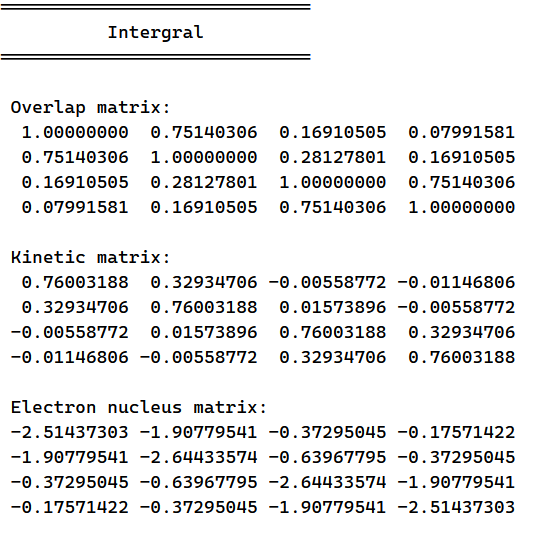
\includegraphics[scale=0.7]{int.png}
	\caption{各种积分}
	\label{Figure 2}
\end{figure}
之后为自洽场迭代过程
\begin{figure}[H]
	\centering
	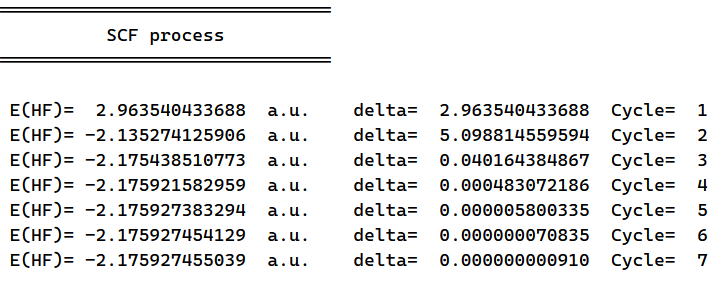
\includegraphics[scale=0.5]{SCF.png}
	\caption{SCF过程}
	\label{Figure 3}
\end{figure}
之后输出电子能量、核排斥能、总能量与轨道能量
\begin{figure}[H]
	\centering
	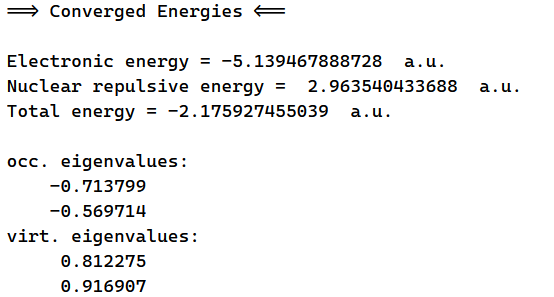
\includegraphics[scale=0.6]{E.png}
	\caption{各种能量}
	\label{Figure 4}
\end{figure}
最后输出系数矩阵与密度矩阵
\begin{figure}[H]
	\centering
	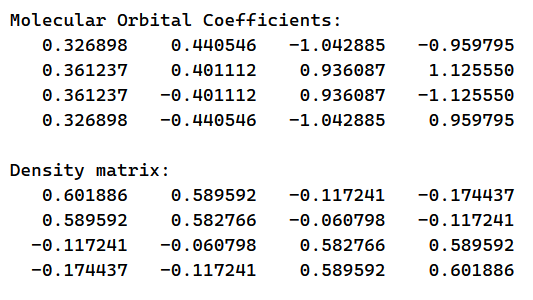
\includegraphics[scale=0.6]{coe.png}
	\caption{系数矩阵与密度矩阵}
	\label{Figure 5}
\end{figure}
以上便是简单的自洽场流程。现在有很多成熟的从头算软件(如Gaussian、orca)可以运用各种帮助收敛的方法(DIIS、damp等)进行SCF过程。

Hartree-Fock方法是量子化学最为基础的方法。由于其采用单电子近似,忽略了电子相关作用,导致其计算能量时有所误差,后面发展的各种post-HF,如组态相互作用(CI)、微扰论(MP)与耦合簇(CC)都是在HF基础上进行了电子相关的修正,其SCF的思想在DFT中也有所体现(KS方程的求解)。因此,熟悉HF的流程,知道HF的推导,是学习量子化学的必经之路。同样的,多数量子化学软件会将自洽场迭代过程展示出来,比如Gaussian,明白了HF方法,便理解了SCF流程,对于监控软件的运行十分有帮助,明白黑箱软件的背后算法,能够更好的使用软件,熟悉Hartree-Fock方法,对理论与计算化学的研究有着非常大的帮助。
\end{document}